% ------------------------------------------------------------------------------
% TYPO3 CMS 6.2 LTS - What's New - Chapter "Istotne zmiany" (English Version)
%
% @author	Michael Schams <schams.net>
% @license	Creative Commons BY-NC-SA 3.0
% @link		http://typo3.org/download/release-notes/whats-new/
% @language	English
% ------------------------------------------------------------------------------
% Chapter: Istotne zmiany
% ------------------------------------------------------------------------------
\section{Istotne zmiany}
\begin{frame}[fragile]
	\frametitle{Istotne zmiany}

	\begin{center}\huge{Rozdział 6:}\end{center}
	\begin{center}\huge{\color{typo3darkgrey}\textbf{Istotne zmiany}}\end{center}

\end{frame}

% ------------------------------------------------------------------------------
% normalize.css
% ------------------------------------------------------------------------------
% http://forge.typo3.org/issues/47920

\begin{frame}[fragile]
	\frametitle{Istotne zmiany}
	\framesubtitle{Normalize.css}

	\begin{itemize}
		\item Interfejs użytkownika w panelu administracyjnym korzysta z \texttt{normalize.css},
			co sprawia, że przeglądarki renderują wszystkie elementy bardziej konsekwentnie i zgodnie z nowoczesnymi standardami
		\item Nowoczesność, zgodność z HTML5, alternatywa dla resetu CSS
		\item Cele \texttt{normalize.css} to:

			\begin{itemize}
				\item zachowywanie użytecznych, domyślnych ustawień przeglądarki a nie ich usuwanie,
				\item normalizacja stylów dla szerokiej gamy elementów HTML,
				\item poprawienie błędów i niespójności popularnych przeglądarek,
				\item zwiększenie użyteczności subtelnymi udoskonaleniami,
				\item wyjaśnienie kodu poprzez użycie komentarzy i szczegółowej dokumentacji.
			\end{itemize}

	\end{itemize}

\end{frame}

% ------------------------------------------------------------------------------
% displayCond options BIT and !BIT
% ------------------------------------------------------------------------------
% http://forge.typo3.org/issues/45514

\begin{frame}[fragile]
	\frametitle{Istotne zmiany}
	\framesubtitle{TCA: opcje displayCond BIT i !BIT}

	\lstset{
		basicstyle=\tiny\ttfamily
	}

	\begin{itemize}
		\item Sprawdzanie wielowartościowych pól w \texttt{displayCond} (bitowe)\newline
			\texttt{BIT}: bit jest ustawiony, \texttt{!BIT}: bit \underline{nie} jest ustawiony
	\end{itemize}

	\begin{columns}[T]

		\begin{column}{.5\textwidth}

			\advance\leftskip+1cm
			Assuming this TCA:

			\lstset{xleftmargin=1cm}

			\begin{lstlisting}
				'content' => array(
				  'label' => '...',
				  'config' => array(
				    'type' => 'check',
				    'items' => array(
				      array('Content A', ''),
				      array('Content B', ''),
				      array('Content C', ''),
				    ),
				  )
				),
			\end{lstlisting}

		\end{column}
		\begin{column}{.5\textwidth}

			Examples:

			\begin{lstlisting}
				'content_a' => array(
				  'label' => '...',
				  'displayCond' => 'FIELD:content:BIT:1',
				  'config' => array(
				    'type' => 'text',
				  )
				),

				'content_b' => array(
				  'label' => '...',
				  'displayCond' => 'FIELD:content:!BIT:2',
				  'config' => array(
				    'type' => 'text',
				  )
				),
			\end{lstlisting}
		\end{column}

	\end{columns}

\end{frame}

% ------------------------------------------------------------------------------
% Automatic language updates for extensions
% ------------------------------------------------------------------------------
% http://forge.typo3.org/issues/43703

\begin{frame}[fragile]
	\frametitle{Istotne zmiany}
	\framesubtitle{Aktualizacje językowe}

	\begin{itemize}
		% \item Extbase Command Controller allows to update translations of extensions for selected languages
		\item Extabase Command Controller wprowadza aktualizacje językowe
		w rozszerzeniach:

			\begin{lstlisting}
				$GLOBALS['TYPO3_CONF_VARS']['SC_OPTIONS']['extbase']
				  ['commandControllers'][] =
				  'TYPO3\\CMS\\Lang\\Command\\LanguageCommandController';
			\end{lstlisting}

		\item Przykład użycia:

			\lstinline!typo3/cli_dispatch.phpsh extbase language:update de,en,fr!

		\item Lista języków oddzielona przecinkami (np. \texttt{en,de,pl}) ogranicza aktualizacje tylko do tych języków
		\item Bez tego argumentu wszystkie języki zawarte w module "Languages" zostaną zaktualizowane

	\end{itemize}

\end{frame}

% ------------------------------------------------------------------------------
% Migrate system extension manuals to reStructuredText
% ------------------------------------------------------------------------------
% http://forge.typo3.org/issues/50052

\begin{frame}[fragile]
	\frametitle{Istotne zmiany}
	\framesubtitle{Rozszerzenia systemowe: instrukcje w formacie ReST}

	\begin{itemize}
		\item wszystkie instrukcje rozszerzeń systemowych są w formacie reStructeredText,
		\item instrukcje w formacie OpenOffice zostały usunięte i nie będą już używane,
		\item ReST jest to łatwa do oczytania składnia WYSIWYG, ze znacznikami zwykłego tekstu jak i system parsowania,
		\item pliki ReST rozszerzeń systemowych są przechowywane w:\newline
			\texttt{typo3/sysext/<extensionkey>/Documentation/*}

		\item Więcej informacji:

			\begin{itemize}
				\item \url{http://de.wikipedia.org/wiki/ReStructuredText}
				\item \url{http://wiki.typo3.org/ReST}
			\end{itemize}

	\end{itemize}

\end{frame}

% ------------------------------------------------------------------------------
% Support custom translation servers for extensions
% ------------------------------------------------------------------------------
% http://forge.typo3.org/issues/50052

\begin{frame}[fragile]
	\frametitle{Istotne zmiany}
	\framesubtitle{Niestandardowe Serwery Tłumaczeń}

	\begin{itemize}
		\item wdrożono obsługę Niestandardowych Serwerów Tłumaczeń rozszerzeń,
		\item dzięki zastosowaniu formatu XLIFF i nowego mechanizmu Signal/Slot stało się to o wiele łatwiejsze,
		\item proponowany serwer tłumaczeń to \textbf{Pootle}

			\begin{itemize}
				\item narzędzie do zarządzania tłumaczeniem online wraz z interfejsem 
				\item napisane w Python/Django
				\item pierwotnie opracowane i wydane przez \url{translate.org.za}
				\item licencja GNU GPL
			\end{itemize}

	\end{itemize}

\end{frame}

% ------------------------------------------------------------------------------
% Support custom translation servers for extensions
% ------------------------------------------------------------------------------
% http://forge.typo3.org/issues/50052

\begin{frame}[fragile]
	\frametitle{Istotne zmiany}
	\framesubtitle{Niestandardowe Serwery Tłumaczeń}

	Przykład: \texttt{EXT:myextension/localconf.php}

	\lstset{
		basicstyle=\tiny\ttfamily
	}

	\begin{lstlisting}
		/**
		 * @var \TYPO3\CMS\Extbase\SignalSlot\Dispatcher $signalSlotDispatcher
		 */
		$signalSlotDispatcher =
		  \TYPO3\CMS\Core\Utility\GeneralUtility::makeInstance(
		    'TYPO3\\CMS\\Extbase\\SignalSlot\\Dispatcher');

		$signalSlotDispatcher->connect(
		  'TYPO3\\CMS\\Lang\\Service\\UpdateTranslationService',
		  'postProcessMirrorUrl',
		  'Company\\Extension\Slots\\CustomMirror',
		  'postProcessMirrorUrl'
		);
	\end{lstlisting}

\end{frame}

% ------------------------------------------------------------------------------
% Support custom translation servers for extensions
% ------------------------------------------------------------------------------
% http://forge.typo3.org/issues/50052

\begin{frame}[fragile]
	\frametitle{Istotne zmiany}
	\framesubtitle{Niestandardowe Serwery Tłumaczeń}

	Przykład: \texttt{EXT:myextension/Classes/Slots/CustomMirror.php}

	\lstset{
		basicstyle=\tiny\ttfamily
	}

	\begin{lstlisting}
		<?php
		namespace Company\Extensions\Slots;
		class CustomMirror {

		  /**
		   * @var string
		   */
		  protected static $extKey = 'myextension';

		  public function postProcessMirrorUrl($extensionKey, &$mirrorUrl) {
		    if ($extensionKey === self::$extKey) {
		      $mirrorUrl = 'http://example.com/typo3-packages/';
		    }
		  }

		}
	\end{lstlisting}

\end{frame}

% ------------------------------------------------------------------------------
% Support custom translation servers for extensions
% ------------------------------------------------------------------------------
% http://forge.typo3.org/issues/50052

\begin{frame}[fragile]
	\frametitle{Istotne zmiany}
	\framesubtitle{Niestandardowe Serwery Tłumaczeń}

	Oczekiwana struktura plików/katalogów na serwerze:

	\begin{lstlisting}
		http://example.com/typo3-packages/
		 `-- <first-letter-of-extension-key>
		     `-- <second-letter-of-extension-key>
		         `-- <extension-key>-l10n
		             |-- <extension-key>-l10n-de.zip
		             |-- <extension-key>-l10n-fr.zip
		             |-- <extension-key>-l10n-it.zip
		             `-- <extension-key>-l10n.xml
	\end{lstlisting}

	Na przykład:

	\begin{lstlisting}
		http://example.com/typo3-packages/m/y/myextension-l10n/myextension-l10n.xml
	\end{lstlisting}

\end{frame}

% ------------------------------------------------------------------------------
% Support custom translation servers for extensions
% ------------------------------------------------------------------------------
% http://forge.typo3.org/issues/50052

\begin{frame}[fragile]
	\frametitle{Istotne zmiany}
	\framesubtitle{Niestandardowe Serwery Tłumaczeń}

	Przykład: \texttt{<extension-key>-l10n.xml}

	\lstset{
		basicstyle=\tiny\ttfamily
	}

	\begin{lstlisting}
		<?xml version="1.0" standalone="yes" ?>
		  <TERlanguagePackIndex>
		    <meta>
		      <timestamp>1374841386</timestamp>
		      <date>2013-07-26 14:23:06</date>
		    </meta>
		    <languagePackIndex>
		    <languagepack language="de">
		      <md5>1cc7046c3b624ba1fb1ef565343b84a1</md5>
		    </languagepack>
		    <languagepack language="fr">
		     <md5>f00f73ae5c43cb68392e6c508b65de7a</md5>
		    </languagepack>
		    <languagepack language="it">
		     <md5>cd59530ce1ee0a38e6309544be6bcb3d</md5>
		    </languagepack>
		  </languagePackIndex>
		</TERlanguagePackIndex>
	\end{lstlisting}

\end{frame}

% ------------------------------------------------------------------------------
% Automatic import of t3d files for extensions
% ------------------------------------------------------------------------------
% http://forge.typo3.org/issues/51437

\begin{frame}[fragile]
	\frametitle{Istotne zmiany}
	\framesubtitle{Automatyczny import t3d}

	\begin{itemize}
		\item rozszerzenia mogą teraz importować pakiety \textbf{inicjalizacyjne t3d} podczas ich instalacji, 
		\item pliki t3d zawierają dane, pliki, relacje itp.,
		\item plik t3d musi nosić nazwę \texttt{data.t3d} i znaleźć się w:\newline
			\texttt{EXT:myextension/Initialisation/}

		\item import jest wykonywany tylko \underline{raz}\newline
			(nawet jeśli rozszerzenie jest później przeinstalowane)

	\end{itemize}

\end{frame}

% ------------------------------------------------------------------------------
% Automatic import of files for extensions
% ------------------------------------------------------------------------------
% http://forge.typo3.org/issues/51446

\begin{frame}[fragile]
	\frametitle{Istotne zmiany}
	\framesubtitle{Automatyczny Import Plików}

	\begin{itemize}
		\item podczas instalacji rozszerzeń mogą one teraz automatycznie importować \textbf{pliki} inicjalizacji,
		\item pliki muszą znaleźć się w:\newline
			\texttt{EXT:myextension/Initialisation/Files/...}
		\item pliki są kopiowane do:\newline
			\texttt{fileadmin/<extensionkey>/}
		\item import jest wykonywany tylko \underline{raz}\newline
			(nawet jeśli rozszerzenie jest później przeinstalowane)

	\end{itemize}

\end{frame}

% ------------------------------------------------------------------------------
% Use an extension as repository
% ------------------------------------------------------------------------------
% http://forge.typo3.org/issues/51835

\begin{frame}[fragile]
	\frametitle{Istotne zmiany}
	\framesubtitle{Użycie rozszerzenia jako repozytorium}

	\begin{itemize}
		\item czasami rozszerzenia są zależne od niestandardowych rozszerzeń lub od rozszerzeń, które nie zostały wydane wraz z oficjalnym Repozytorium Rozszerzeń TYPO3 (TER),
		\item aby rozwiązać ten problem, rozszerzenia mogą być teraz dostarczane wraz z innymi rozszerzeniami,
		\item te muszą być umieszczone w (po rozpakowaniu):\newline
			\texttt{EXT:myextension/Initialisation/Extensions/...}

		\item po instalacji rozszerzenia są kopiowane do:\newline
			\texttt{typo3conf/ext/}

		\item po tym problem zależności rozszerzeń jest rozwiązany
	\end{itemize}

\end{frame}

% ------------------------------------------------------------------------------
% CLI command to install/uninstall extensions
% ------------------------------------------------------------------------------
% http://forge.typo3.org/issues/51629

\begin{frame}[fragile]
	\frametitle{Istotne zmiany}
	\framesubtitle{Instalowanie/odinstalowywanie rozszerzeń przez CLI}

	\begin{itemize}
		\item Instalowanie i odinstalowywanie rozszerzeń za pomocą interfejsu wiersza poleceń (CLI)
		\item Przykłady:
			\lstinline!typo3/cli_dispatch.phpsh extbase extension:install <extensionkey>!
			\lstinline!typo3/cli_dispatch.phpsh extbase extension:uninstall <extensionkey>!

		\item Uwaga: do tego jest wymagany użytkownik panelu administracyjnego \textbf{\_cli\_lowlevel}
	\end{itemize}

\end{frame}

% ------------------------------------------------------------------------------
% Enable/disable cascading deletion of child elements
% ------------------------------------------------------------------------------
% http://forge.typo3.org/issues/50391

\begin{frame}[fragile]
	\frametitle{Istotne zmiany}
	\framesubtitle{Kaskadowe tłumaczenie elementów potomnych}

	\begin{itemize}
		\item TCA oferuje teraz możliwość włączenia/wyłączenia kaskadowego usuwania elementów potomnych, 
		\item relacje muszą mieć typ "\textbf{inline}",
		\item domyślną wartością jest \texttt{TRUE} (włączono usuwanie rekordów potomnych typu inline),
		\item przykład (wyłączenie usuwania rekordów potomnych typu inline):

			\begin{lstlisting}
				...
				'type' => 'inline',
				'foreign_table' => ...,
				  'behaviour' => array(
				    'enableCascadingDelete' => 0
				  )
				  ...
				)
				...
			\end{lstlisting}

	\end{itemize}

\end{frame}

% ------------------------------------------------------------------------------
% Multiple category fields per table
% ------------------------------------------------------------------------------
% http://forge.typo3.org/issues/51921

\begin{frame}[fragile]
	\frametitle{Istotne zmiany}
	\framesubtitle{Wielokrotne pola kategorii w tabeli}

	\begin{itemize}
		\item W TYPO3 < 6.2, możliwe jest tylko \underline{jedno} wywołanie \texttt{makeCategorizable()} na tabelę
			(wielokrotne wywołanie mogłoby zastąpić wcześniejsze deklaracje pól kategorii)
		\item Od TYPO3 >= 6.2, wielokrotne pola kategorii w tabeli są możliwe
		\item Przykład:

			\begin{lstlisting}
				\TYPO3\CMS\Core\Utility\ExtensionManagementUtility::makeCategorizable(
				  $extensionKey,
				  $tableName,
				  $fieldName = 'categories',
				  $options = array(
				  	'label' => 'my category'
				  )
				);
			\end{lstlisting}

		\item Etykiety dla pól kategorii można ustawić w tablicy \texttt{\$options}

	\end{itemize}

\end{frame}

% ------------------------------------------------------------------------------
% Backend layout data providers
% ------------------------------------------------------------------------------
% http://forge.typo3.org/issues/37208

\begin{frame}[fragile]
	\frametitle{Istotne zmiany}
	\framesubtitle{Dostawcy wyglądu elementów (ang. BE Layout) w panelu administracyjnym}

	\begin{itemize}
		\item W TYPO3 < 6.2, wyglądy elementów (ang. BE) są przechowywane w bazie danych tak jak zwykłe rekordy,
		\item od TYPO3 >= 6.2 \emph{dostawcy takich danych} mogą być zdefiniowani\newline
			\small(na przykład aby włączyć rozszerzenia, które są oferowane wraz z własnymi definicjami wyglądu BE i które są przechowywane w plikach),\normalsize

		\item dostawcy takich danych muszą napisać implementację interfejsu zdefiniowaną w klasie:\newline
			\smaller\texttt{
				TYPO3\textbackslash\textbackslash
				CMS\textbackslash\textbackslash
				Backend\textbackslash\textbackslash
				View\textbackslash\textbackslash
				BackendLayout\textbackslash\textbackslash
				DataProviderInterface}\normalsize

		\item i zarejestrować ją za pomocą instrukcji:

			\begin{lstlisting}
				$GLOBALS['TYPO3_CONF_VARS']['SC_OPTIONS']
				  ['BackendLayoutDataProvider'][$_EXTKEY] = 'Classname';
			\end{lstlisting}


	\end{itemize}

\end{frame}

% ------------------------------------------------------------------------------
% Backend layout data providers
% ------------------------------------------------------------------------------
% http://forge.typo3.org/issues/37208

\begin{frame}[fragile]
	\frametitle{Istotne zmiany}
	\framesubtitle{Layout'y dostawców danych w panelu administracyjnym}

	\begin{itemize}
		\item Nowe funkcje API do obsługi panelu administracyjnego dostawców danych:

			\begin{lstlisting}
				'itemsProcFunc' => 'TYPO3\\CMS\\Backend\\View\\
				  BackendLayoutView->addBackendLayoutItems'
			\end{lstlisting}

			\begin{lstlisting}
				getBackendLayoutView()->getSelectedCombinedIdentifier($id);
				getBackendLayoutView()->getSelectedBackendLayout();
			\end{lstlisting}

		\item Nowa opcja PageTSconfig do wykluczania layout'ów panelu administracyjnego:

			\begin{lstlisting}
				options.backendLayout.exclude = default_1, my_extension__headerLayout
			\end{lstlisting}

	\end{itemize}

\end{frame}

% ------------------------------------------------------------------------------
% Filter for multiple value selector
% ------------------------------------------------------------------------------
% http://forge.typo3.org/issues/49739

\begin{frame}[fragile]
	\frametitle{Istotne zmiany}
	\framesubtitle{Selektor wielokrotnego wyboru (1)}

	\lstset{
		basicstyle=\tiny\ttfamily
	}

	\begin{itemize}
		\item filtrowanie dostępnych pozycji w elemencie wielokrotnego wyboru,
		\item np: użytkownik może wybrać z rozwijanej listy aktywne pole tekstowe dla indywidualnie filtrowanych słów i wstępnie zdefiniowanych słów do wyszukiwania,
		%\item For example: enable a text field for individual word filter and pre-define search words a user can select from a drop down box

		\item aby skorzystać z tej funkcji ustaw odpowiednio TCA\newline
			(np. w pliku \texttt{typo3conf/extTables.php}):


			\begin{lstlisting}
				$GLOBALS['TCA']['fe_users']['columns']['usergroup']['config']
				  ['enableMultiSelectFilterTextfield'] = TRUE;
				$GLOBALS['TCA']['fe_users']['columns']['usergroup']['config']
				  ['multiSelectFilterItems'] = array(
				  array('',     'show all'),  // no filter
				  array('test', 'test'),      // first value: filter, second value: label
				  array(
				    'TYPO3',
				    'LLL:EXT:myext/Resources/Private/Language/locallang_db.xlf:tx_myext.label.typo3'
				  ),
				);
			\end{lstlisting}

	\end{itemize}

\end{frame}

% ------------------------------------------------------------------------------
% Filter for multiple value selector
% ------------------------------------------------------------------------------
% http://forge.typo3.org/issues/49739

\begin{frame}[fragile]
	\frametitle{Istotne zmiany}
	\framesubtitle{Selektor wielokrotnego wyboru (2)}

	\begin{itemize}
		\item Dostępne są dwie opcje:

			\begin{itemize}
				\item wybierz wstępnie zdefiniowane wartości z rozwijanej listy,
				\item wpisz szukane słowo/filtr do pola wprowadzania.
			\end{itemize}

		\item Wynik może wyglądać tak:
	\end{itemize}

	\begin{figure}
		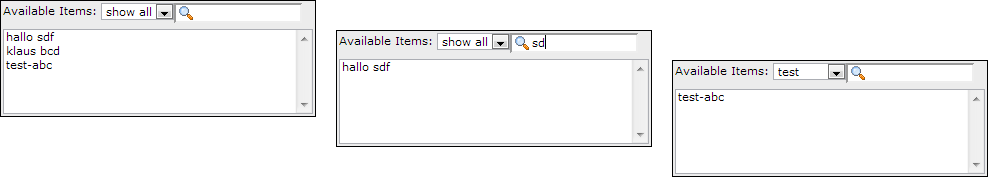
\includegraphics[width=1\linewidth]{Images/InDepthChanges/MultipleValueSelector.png}
	\end{figure}

\end{frame}

% ------------------------------------------------------------------------------
% Improved caching framework by introducing cache groups
% (slide added in March 2014)
% ------------------------------------------------------------------------------
% http://forge.typo3.org/issues/54991

\begin{frame}[fragile]
	\frametitle{Istotne zmiany}
	\framesubtitle{Grupy pamięci podręcznej (1)}

	\begin{itemize}
		\item Jądro TYPO3 wykorzystuje dwa typy pamięci podręcznej:

			\begin{itemize}
				\item \textbf{systemowa pamięć podręczna}:
				class loading cache, configuration cache, l10n\_cache, extbase\_object, extbase\_reflection etc.
				\item \textbf{frontend'owa pamięć podręczna}:
				cHash cache, page cache, page section cache
			\end{itemize}

		\item w TYPO3 < 6.2, \textit{clear all caches} opróznia \underline{całą} pamięć podręczną, co nie jest idealne,

		\item w TYPO3 >= 6.2, rdzeń wykorzystuje dwie grupy pamięci podręcznej:\newline
			"\textbf{pages}" związana z pamięcią podręczną wszystkich stron i "\textbf{system}", która jest stosowana w czasie kompilacji i buforowania konfiguracji

	\end{itemize}

	\begin{figure}
		
\includegraphics[width=0.5\linewidth]{Images/InDepthChanges/CacheGroups.png}
	\end{figure}

\end{frame}

% ------------------------------------------------------------------------------
% Improved caching framework by introducing cache groups
% (slide added in March 2014)
% ------------------------------------------------------------------------------
% http://forge.typo3.org/issues/54991

\begin{frame}[fragile]
	\frametitle{Istotne zmiany}
	\framesubtitle{Grupy pamięci podręcznej (2)}

	\lstset{
		basicstyle=\tiny\ttfamily
	}

	\begin{itemize}

		\item Istotne opcje konfiguracji:\newline
			\smaller(w plikach: \texttt{LocalConfiguration.php}/\texttt{DefaultConfiguration.php})\normalsize

			\begin{lstlisting}
			'cache_hash' => array(
			  'frontend' => 'TYPO3\CMS\Core\Cache\Frontend\VariableFrontend',
			  'backend' => 'TYPO3\CMS\Core\Cache\Backend\Typo3DatabaseBackend',
			  'options' => array(),
			  'groups' => array('pages', 'all')
			),
			\end{lstlisting}

		\item "\textit{Flush all caches}" nie odświeża systemowej pamięci podręcznej
			(tylko "Clear Configuration Cache" lub instalator czyści tę pamięć)
		\item Nowa opcja userTSconfig  umożliwia zwykłym użytkownikom czyszczenie systemowej pamięci podręcznej:\newline
			\smaller \texttt{options.clearCache.system = 1}\normalsize

		\breakingchange

	\end{itemize}

\end{frame}

% ------------------------------------------------------------------------------
% TCA: limit number of ticked checkboxes
% (slide added in March 2014)
% ------------------------------------------------------------------------------
% http://forge.typo3.org/issues/55187
% http://forge.typo3.org/issues/55188 (documentation: TCA reference)

\begin{frame}[fragile]
	\frametitle{Istotne zmiany}
	\framesubtitle{TCA: Liczba zaznaczonych pól wyboru}

	\lstset{
		basicstyle=\tiny\ttfamily
	}

	\begin{itemize}
		\item TCA umożliwia sprawdzenie liczby zaznaczonych pól wyboru

			\begin{itemize}
				\item \texttt{maximumRecordsChecked}:\newline
					limit liczby rekordów dla całego systemu
				\item \texttt{maximumRecordsCheckedInPid}:\newline
					limit ilości rekordów dla całego PID (parent ID)
			\end{itemize}

		\item Jeżeli użytkownik BE przekroczy liczbę
		maksymalną to dodatkowe zaznaczenie będzie odrzucone dopóki nie zostanie
		odznaczony wcześniejszy rekord,
		\item Przykład:

			\begin{lstlisting}
				$tcaConfiguration = array(
				  'type' => 'check',
				  'eval' => 'maximumRecordsChecked',
				  'validation' => array(
				    'maximumRecordsChecked' => 5
				  )
				);
			\end{lstlisting}

	\end{itemize}

\end{frame}

% ------------------------------------------------------------------------------
% TCA: Introduce MM_oppositeUsage property
% (slide added in March 2014)
% ------------------------------------------------------------------------------
% http://forge.typo3.org/issues/56061
% http://forge.typo3.org/issues/56123 (documentation: TCA reference)

\begin{frame}[fragile]
	\frametitle{Istotne zmiany}
	\framesubtitle{TCA: właściwość \texttt{MM\_oppositeUsage}}

	\lstset{
		basicstyle=\tiny\ttfamily
	}

	\begin{itemize}
		\item podczas kopiowania rekordu \texttt{sys\_category} jest tworzona nowa referencja MM, ale bez ustawienia pola "fieldname",
		\item Wartość ta jest zdefiniowana w przeciwnej encji z właściwością \texttt{MM\_match\_fields}, która niestety nie jest dostępna, ale nie może być dostępna,
		\item aby rozwiązać ten problem, do TCA wprowadzono nową właściwość \texttt{MM\_oppositeUsage}:

			\begin{lstlisting}
				'config' => array(
				  'allowed' => '*',
				  'MM' => 'tx_myextension_first_second_mm',
				  'MM_oppositeUsage' => array(
				    'tt_content' => array('somefield'),
				    'tx_myextension_domain_model' => array('some_property'),
				  ),
				),
			\end{lstlisting}

	\end{itemize}

\end{frame}

% ------------------------------------------------------------------------------
% Miscellaneous
% ------------------------------------------------------------------------------
% http://forge.typo3.org/issues/49037 (Custom record list in element browser)
% http://forge.typo3.org/issues/36505 (Increase size of be_groups.subgroup field)
% http://forge.typo3.org/issues/49270 (Merge extensions TS/Template)

\begin{frame}[fragile]
	\frametitle{Istotne zmiany}
	\framesubtitle{Różne}

	\begin{itemize}

		\item \textbf{Lista niestandardowych rekordów:}\newline
			\small
				Instancja listy niestandardowych rekordów może być używana w przeglądarce elementów, aby zastąpić domyślną listę rekordów
			\normalsize

		\item \textbf{Więcej podgrup:}\newline
			\small
				Atrybut \texttt{subgroup} w bazie danych w tabeli \texttt{be\_groups} zmieniony z \texttt{varchar(250)} na \texttt{text}, co pozwala na znacznie więcej podgrup (użytkowników/grup panelu administracyjnego)
			\normalsize

		\item \textbf{Rozszerzenia TS/Połączony template:}\newline
			\small
				Technicznie, "WEB > Template" było rozprowadzone na kilka rozszerzeń (tstemplate\_ceditor, tstemplate\_info, tstemplate\_objbrowser i tstemplate\_analyzer). Te rozszerzenia są teraz połączone w jedno: "tstemplate"
			\normalsize

	\end{itemize}
	
\end{frame}

% ------------------------------------------------------------------------------
% Miscellaneous
% ------------------------------------------------------------------------------
% http://forge.typo3.org/issues/49721 (Add label_userFunc_options support to BackendUtility)
% http://forge.typo3.org/issues/50441 (Add a timestamp when downloading an extension)
% http://forge.typo3.org/issues/51352 (Force saltedpasswords for Backend)

\begin{frame}[fragile]
	\frametitle{Istotne zmiany}
	\framesubtitle{Różne}

	\begin{itemize}

		\item \textbf{label\_userFunc\_options:}\newline
			\small
				Wsparcie dla \texttt{label\_userFunc\_options} dodane do \texttt{BackendUtility}
			\normalsize

		\item \textbf{Extension filename:}\newline
			\small
				Podczas pobierania rozszerzenia w Menadżerze Rozszerzeń, nazwa pliku otrzymuje znacznik czasowy (rok, miesiąc, dzień i czas):\newline
				\texttt{<extensionKey>\_<version>\_<timestamp>.zip}\newline
				\texttt{myextension\_1.0.0\_201312102359.zip}
			\normalsize

		\item \textbf{EXT:saltedpasswords:}\newline
			\small
				Rozszerzenie EXT:saltedpasswords jest wymaganym rozszerzeniem systemu i jest teraz domyślnie włączone.
				Zmusza to znaki zaszyfrowane metodą "salt" do uwierzytelnienia w panelu administracyjnym. Instalator sprawdza ustawienia i dostosowuje je w razie potrzeby.
			\normalsize

	\end{itemize}
	
\end{frame}

% ------------------------------------------------------------------------------
% Miscellaneous
% ------------------------------------------------------------------------------
% http://forge.typo3.org/issues/51138 (Allow SignalSlots to modify arguments)
% http://forge.typo3.org/issues/31996 (Transfer query parameters in preview)
% http://forge.typo3.org/issues/52630 (TCEforms PlaceHolder works recursively now)

\begin{frame}[fragile]
	\frametitle{Istotne zmiany}
	\framesubtitle{Różne}

	\begin{itemize}

		\item \textbf{SignalSlots do zmodyfikowania argumentów:}\newline
			\small
				Argumenty przekazywane do dispatcher'a SignalSlots mogą teraz być modyfikowane. Dispatcher zwraca (zmodyfikowane) argumenty otrzymane w celu zachowania nienaruszonych łańcuchów.
			\normalsize

		\item \textbf{Podgląd workspace:}\newline
			\small
				Parametry zapytania są przekazywane teraz do podglądu workspace'a. Był to problem w TYPO3 < 6.2, gdzie rozszerzenia przekazujące niestandardowe parametry nie działają prawidłowo
			\normalsize

		\item \textbf{Funkcja TCEforms PlaceHolder:}\newline
			\small
				Wprowadzona w TYPO3 CMS 4.7, funkcja PlaceHolder z TCEforms działa od teraz rekursywnie (e.g. \texttt{\_\_row|uid\_foreign|field}).
			\normalsize

	\end{itemize}
	
\end{frame}

% ------------------------------------------------------------------------------
% Miscellaneous
% ------------------------------------------------------------------------------
% http://forge.typo3.org/issues/14730 (Support for proxy NTLM authentication)
% http://forge.typo3.org/issues/49667 (Enable double-resolution icons in SpriteGenerator)

\begin{frame}[fragile]
	\frametitle{Istotne zmiany}
	\framesubtitle{Różne}

	\begin{itemize}

		\item \textbf{Ikony z podwojoną rozdzielczością:}\newline
			\small
				SpriteManager obsługuje od teraz ikony w wysokiej rozdzielczości: generuje on drugą ikonę w podwojonej rozdzielczości (drugi plik z  przyrostkiem "@x2.png"). CSS3 zapewnia, że plik w wysokiej rozdzielczości jest ładowany na urządzeniach które ją wspierają. (nie ma to wpływu na działanie innych urządzeń).
			\normalsize

		\item \textbf{Uwierzytelnianie proxy NTLM:}\newline
			\small
				Dodane wsparcie dla uwierzytelniania proxy NTLM (\textbf{NT} \textbf{L}AN \textbf{M}anager: zestaw protokołów bezpieczeństwa Microsoft'u). Ta funkcja może być aktywowana w instalatorze:\newline
			\normalsize
			\smaller
				\texttt{\$GLOBALS['TYPO3\_CONF\_VARS']['SYS']['curlProxyNTLM']}\newline
				\emph{(przy okazji: ta funkcja została wprowadzona ponad 8 lat temu :-))}
			\normalsize

	\end{itemize}
	
\end{frame}

% ------------------------------------------------------------------------------
% Miscellaneous
% (slide added in March 2014)
% ------------------------------------------------------------------------------
% http://forge.typo3.org/issues/14730 (Support for proxy NTLM authentication)

\begin{frame}[fragile]
	\frametitle{Istotne zmiany}
	\framesubtitle{Różne}

	\begin{itemize}

		\item \textbf{Domyślne cookieHttpOnly:}\newline
			\small
				Tworzenie ciasteczka sesji dostępnej tylko za pośrednictwem protokołu HTTP, \texttt{cookieHttpOnly} jest teraz włączone domyślnie.\newline
				Oznacza to, że ciasteczka "fe\_typo\_user" i "be\_typo\_user" nie będą dostępne dla języków skryptowych (np. JavaScript), co wzmacnia ochronę przed atakami XSS (\textit{cross site scripting}), chociaż niektóre starsze przeglądarki nie obsługują tej techniki.
			\normalsize

		\item \textbf{Czyszczenie tabeli w bazie danych:}\newline
			\small
				Następujące atrybuty zostały usunięte z tabeli \texttt{tt\_content} (nie używanej od TYPO3 4.0):
				\texttt{text\_align}, \texttt{text\_face}, \texttt{text\_size}, \texttt{text\_color}, \texttt{text\_properties}.
			\normalsize

	\end{itemize}
	
\end{frame}

% ------------------------------------------------------------------------------
% Miscellaneous
% (slide added in March 2014)
% ------------------------------------------------------------------------------
% https://forge.typo3.org/issues/55190 (Move Tidy functionality to a TER extension)

\begin{frame}[fragile]
	\frametitle{Istotne zmiany}
	\framesubtitle{Różne}

	\begin{itemize}

		\item \textbf{HTML Tidy usunięty:}\newline
			\small
				Funkcjonalność \textit{HTML Tidy} została usunięta z rdzenia TYPO3. Może być to łatwo wprowadzone ponownie przez użycie EXT:tidy z TER'a.
			\normalsize

		\item \textbf{dontSetCookie usunięty:}\newline
			\small
				Ze względu na fakt, że ciasteczko "fe\_typo\_user" jest ustawione tylko gdy potrzeba (lecz nie zawsze), instalator opcji \texttt{dontSetCookie} jest nieistotny i został usunięty.
			\normalsize

		\item \textbf{Skrypt "wizard" usunięty:}\newline
			\small
				Usunięcie następujących skryptów "wizard":
				\texttt{typo3/wizard\_add.php}, \texttt{typo3/wizard\_colorpicker.php}, \texttt{typo3/wizard\_edit.php}, \texttt{typo3/wizard\_forms.php}, \texttt{typo3/wizard\_list.php}, \texttt{typo3/wizard\_rte.php}, \texttt{typo3/wizard\_table.php}
			\normalsize

	\end{itemize}
	
\end{frame}

% ------------------------------------------------------------------------------

